\documentclass{article}

\usepackage[final]{neurips_2019}
\usepackage{amsmath}
\usepackage[utf8]{inputenc}
\usepackage[T1]{fontenc}
\usepackage{hyperref}
\usepackage{url}
\usepackage{booktabs}
\usepackage{amsfonts}
\usepackage{nicefrac}
\usepackage{microtype}
\usepackage{graphicx}
\usepackage{xcolor}
\usepackage{lipsum}
\usepackage{booktabs}
\usepackage{xcolor}
\usepackage{float}
\setlength{\textfloatsep}{10pt}
\setlength{\intextsep}{10pt}
\newcommand{\note}[1]{\textcolor{blue}{{#1}}}

\title{
    Test-Time Training on Binary Sub-Problems\\
  \vspace{1em}
  \small{\normalfont Stanford CS224N Custom Project}  % Select one and delete the other
}

\author{
  Andrew Sung \\
  Department of Computer Science \\
  Stanford University \\
  \texttt{drewsung@stanford.edu} \\
  \And
  Darrow Hartman \\
  Department of Computer Science \\
  Stanford University \\
  \texttt{darrowrh@stanford.edu} \\
  \And
  Leo Li \\
  Department of Computer Science \\
  Stanford University \\
  \texttt{leo0912@stanford.edu}
}

\raggedbottom
\begin{document}

\maketitle
 
\begin{abstract}
Recent work on test-time training (TTT) has shown that large language models (LLMs) can improve on individual problems by continuing to learn at inference time. However, existing approaches like TTT-Discover rely on continuous reward signals, making them unsuitable for binary problems where the answer is either correct or incorrect. We propose a consensus as ground truth approach to test-time training for improving performance on binary verification problems. Our method prompts the model to decompose a hard target problem into easier subproblems, filters them using a self-consistency window of 60-80\% to ensure pseudo-label reliability and appropriate difficulty calibration, and trains on the resulting curriculum using Group Relative Policy Optimization (GRPO). We evaluate our approach on a Tier 3 FrontierMath arithmetic geometry problem where the initial model (gpt-oss-120b) achieves a solve rate of 0.67\%. After training on 50 self-generated subproblems for 50 optimization steps, the 500-sample solve rate increases to 30.6\%, a roughly $46\times$ improvement that substantially outperforms GPT-5.4 Medium Thinking (11.20\%). Further gains are achieved by resampling subproblems from the improved checkpoint and continuing training, reaching 32.4\% at step 90. Our analysis reveals that the training procedure exhibits some robustness to noisy pseudo-labels, with the model in some cases recovering correct answers despite being supervised with incorrect targets. We also identify pseudo-label reliability and subproblem quality as key bottlenecks, with approximately 50\% of assigned labels disagreeing with frontier-model consensus, pointing to important directions for future work. Our code is available at \url{https://github.com/Darrow8/ttt-binary}
\end{abstract}


\section{Key Information to include}
\begin{itemize}
    \item Mentor: Chenglei Si
    \item External Collaborators (if you have any): Thinking Machines Lab
    % \item Sharing project: N/A
    % \item Late Days (if you are using any):
    % \\[0.25em] % comment out this entire late days table if you're not using late days for the final report
    % \small
    % \begin{tabular}{l c}
    %     \toprule
    %     \textbf{Team member} & \textbf{Late days remaining} \\
    %     \midrule
    %     <Name 1> & <> \\
    %     <Name 2> & <> \\
    %     <Name 3> & <> \\
    %     \midrule
    %     Total pooled & <> \\
    %     Team size & <> \\
    %     Late days applied for the report & <> \\
    %     \bottomrule
    % \end{tabular}
\end{itemize}

% {\color{red} This template does not contain the full instruction set for this assignment; please refer back to the milestone instructions PDF.}

\section{Introduction}
% \lipsum[1][1-9] 
Consider a student trying to solve a problem they have no idea how to approach. Rather than staring at the problem for hours, a more effective strategy is to break the problem down: solve simpler cases first, build intuition from those cases, and gradually work up to the hard problem. This is the core idea behind our approach to test-time training for large language models (LLMs). 
 
Recent work on test-time training showed that LLMs can improve on individual problems by continuing to learn at inference, rather than relying solely on frozen pretrained weights. TTT-Discover \cite{tttdiscover} showed that running RL at test time on a single problem instance can achieve SoTA results on scientific discovery tasks like the Erd\H{o}s minimum overlap bound, where each candidate solution receives a continuous scalar reward reflecting its quality.
 
However, many important problem classes (such as mathematical reasoning, code generation, formal verification) offer only \textit{binary} feedback: the answer is correct or it is not. Extending TTT-Discover to this setting is fundamentally difficult. Under binary rewards $R \in \{0, 1\}$, when a problem is too difficult for the model to ever produce a correct solution, every rollout in a GRPO group receives the same reward of $0$. The core challenge is that binary problems offer no partial credit: there is no way to distinguish a rollout that was close to correct, from one that was completely wrong.
 
We address this by generating a curriculum of easier subproblems that target the skills needed for the hard problem. We prompt the model to decompose the target into simpler variants, validate them using majority-vote consensus, and train on them with GRPO \cite{deepseekmath}. On a Tier 3 FrontierMath problem where the base model succeeds $0.67\%$ of the time, training on 50 self-generated subproblems increased the success rate to $30.6\%$---a roughly $46\times$ improvement that substantially outperforms GPT-5.4 Medium Thinking ($11.20\%$) under the same evaluation protocol. We further show that iteratively resampling subproblems from the improved checkpoint and continuing training yields additional gains, reaching $32.4\%$. Our analysis also reveals that subproblem quality is a critical factor: simply replacing five poorly posed multi-part subproblems with single-answer variants nearly tripled the solve rate, and post-training solutions consistently exhibit reasoning traces absent from the base model's outputs.

\section{Related Work}

Our approach sits at the intersection of four research threads: test-time reinforcement learning, consensus-based training without labels, synthetic task generation, and curriculum design for RL. We organize this section around the logical arc of our pipeline—starting from the binary reward gap that motivates our work, then the need for appropriately difficult subproblems, the challenge of labeling them without ground truth, and finally the optimization procedure we build on.

\subsection{Test-Time RL and the Binary Reward Gap}
\label{sec:ttt_rl}

TTT-Discover \cite{tttdiscover} demonstrated that RL at test time on a single problem instance can achieve state-of-the-art results, surpassing both the human best and AlphaEvolve on the Erd\H{o}s minimum overlap problem. The key enabler is \textit{continuous reward}: every candidate solution receives a scalar score, so rollout groups always exhibit non-zero reward variance and policy gradients remain well-defined. Our work directly extends TTT-Discover to the binary reward regime, where this assumption breaks down. Under binary rewards $R \in \{0, 1\}$, a problem that is too hard for the model produces rollout groups in which every sample scores 0, collapsing all advantages to zero and eliminating the learning signal entirely. Rather than attempting to run RL on the target problem directly, we restore reward variance by constructing a subproblem curriculum where the model has non-trivial success rates—the design of which is informed by the curriculum RL literature discussed in \S\ref{sec:curriculum}.

\subsection{Curriculum RL and Difficulty Calibration}
\label{sec:curriculum}

Given that binary rewards require the model to succeed on at least some rollouts, the natural question is: \textit{how difficult should the training problems be?} VCRL \cite{vcrl} showed that RL training signal is maximized when the model succeeds roughly 50\% of the time, since this is where reward variance—and therefore gradient magnitude—peaks. TTC-RL \cite{tticrl} and curriculum RL for reasoning \cite{curriculumrl} operationalize this insight by building easy-to-hard task progressions.

These results directly shaped our subproblem filtering criterion. We retain only subproblems where the model's self-consistency rate falls in the 60--80\% range, targeting the difficulty frontier where GRPO \cite{deepseekmath} updates are most informative. The asymmetry of our window—shifted above the theoretically optimal 50\%---reflects a dual requirement: we need not only sufficient reward variance for learning, but also enough agreement among sampled solutions to trust the majority answer as a pseudo-label (\S\ref{sec:rl_testset}). Problems below 60\% are both too hard for effective learning and too unreliable for pseudo-labeling; problems above 80\% are too easy to provide meaningful gradient signal.

\subsection{Synthesizing Training Tasks Without Ground Truth}
\label{sec:synth}

Our approach requires generating subproblems that the model can partially solve, but these generated problems lack ground-truth answers. This challenge—creating verifiable training signal from unverifiable sources—has been addressed in different ways by recent work, each relying on a form of external verification that we lack.

Golden Goose \cite{goldengoose} synthesizes over 700k verifiable RL tasks from unverifiable internet text by converting fill-in-the-middle exercises into multiple-choice questions with unambiguous correct answers. Their tasks have correctness \textit{by construction}. STP \cite{stp} takes a self-play approach in formal theorem proving: a \textit{conjecturer} generates theorems calibrated to be barely provable by the current \textit{prover}, which then trains on them via expert iteration. STP's difficulty-targeting mechanism—generating problems the prover can barely solve—is conceptually aligned with our self-consistency filtering. However, STP leverages formal verifiers (Lean, Isabelle) to obtain ground-truth correctness signals.

Our setting differs from both: we have neither constructed-by-design correctness nor access to a formal verifier. This forces us to rely on consensus-based pseudo-labels as an approximate substitute for ground truth, which introduces the label noise we analyze in \S6.2.

\subsection{Consensus-Based Training and Pseudo-Labels}
\label{sec:rl_testset}

To label our generated subproblems, we repurpose the majority-vote consensus mechanism same as TTRL \cite{ttrl}, which performs RL across an entire test set without ground-truth labels by using agreement across rollouts as pseudo-rewards. A critical assumption in TTRL is that the base model can occasionally produce correct solutions to bootstrap from. On problems where the model's pass rate is near zero—as in our target problem (0.67\% solve rate)—this assumption fails and TTRL-style training on the target problem directly produces no useful signal. Our subproblem generation step is designed precisely to sidestep this limitation: by constructing problems the model \textit{can} partially solve, we create the conditions under which consensus-based pseudo-labels become reliable. We include TTRL-style direct RL on the target problem as a baseline to confirm this reasoning.

Concurrently, Intuitor \cite{intuitor} eliminates external rewards entirely by using the model's own confidence—termed \textit{self-certainty}—as the sole reward signal within GRPO, matching standard GRPO performance on mathematical benchmarks while generalizing better to out-of-domain tasks. While Intuitor operates on problems the model can already attempt, their finding that self-certainty is a viable reward signal is directly relevant to the pseudo-label reliability bottleneck we identify in our analysis (\S6.2): replacing or supplementing majority-vote labels with confidence-based rewards could reduce the approximately 50\% label error rate we observe, and we view this as a promising direction for future work.


\section{Approach}
%\lipsum[1][1-9] 
\subsection{Self-Consistency Filtering}
 
A central challenge in our approach is that the generated subproblems have no ground-truth answers, we create them precisely because they are novel variants of the target problem. We address this by using \emph{self-consistency} as a proxy for both correctness and difficulty calibration.
 
For each candidate subproblem, we sample 10 solutions from \texttt{gpt-oss-120b} at temperature 0.7 and extract the final numerical answer from each. We then compute the \emph{modal-answer frequency}---the fraction of samples that agree on the most common answer. We retain a subproblem only if this frequency falls between 60\% and 80\%, and we adopt the modal answer as the pseudo-label for GRPO training.
 
This filtering criterion serves two purposes:
 
When a large majority of independent samples converge on the same answer, it is unlikely to be a coincidence---the model is ``agreeing with itself'' across diverse reasoning paths. This is the same intuition behind majority-vote decoding \cite{selfconsistency}, but repurposed here for label generation rather than answer selection. Problems below the 60\% threshold exhibit too little agreement for us to trust any single answer as a pseudo-label, increasing the risk of training on incorrect targets.
 
VCRL \cite{vcrl} demonstrates that RL training signal is maximized when the model succeeds roughly 50\% of the time, since this is where reward variance---and therefore gradient magnitude---is highest. Our 60--80\% acceptance window targets a similar regime: problems in this range are ones the model can solve but not trivially, ensuring each subproblem sits near the model's learning frontier. Problems above 80\% are too easy to provide meaningful gradient signal, while problems below 60\% are both too hard for effective learning and too unreliable for pseudo-labeling. The asymmetry of our window (shifted above 50\%) reflects the fact that we need sufficient agreement to trust the pseudo-label, not just maximal variance.
 
In practice, this filtering is quite selective---approximately one in seven candidate subproblems passes, with roughly 586 candidates discarded during generation of our 100 valid subproblems.

\subsection{Group Relative Policy Optimization}
 
We optimize the model on validated subproblems using Group Relative Policy Optimization (GRPO) \cite{grpo}. Unlike PPO \cite{ppo}, which requires a separately trained critic network for variance reduction, GRPO computes advantages relative to a group of sampled rollouts, making it lightweight enough for test-time adaptation where we cannot afford auxiliary model components. Concretely, for each subproblem $q$ we sample a group of $G$ responses $\{o_1, \ldots, o_G\}$ from the current policy $\pi_\theta$, assign each a reward $r_i$ based on exact-match correctness, and compute normalized advantages $\hat{A}_i = (r_i - \text{mean}(\mathbf{r})) / (\text{std}(\mathbf{r}) + \epsilon)$. The policy is updated via a clipped surrogate objective with a KL penalty against the reference policy $\pi_{\text{ref}}$ to prevent the model from drifting too far from its pretrained capabilities. We assign a reward of $1.0$ when the extracted answer matches the pseudo-label and $0.01$ for any response that produces a boxed final answer regardless of correctness; this formatting reward ensures nonzero reward variance even in groups where no response is fully correct. Critically, this optimization procedure is designed to work in concert with our self-consistency filtering (\S4.1): because we only retain subproblems where the model solves 60--80\% of samples, each GRPO group is likely to contain a mixture of correct and incorrect rollouts, so the normalized advantages are well-defined and gradient updates are meaningful. Training directly on the target problem---where the base model's success rate is 0.67\%---would cause nearly every group to consist entirely of failures, collapsing all advantages to zero and producing no learning signal.

\section{Experiments}

\subsection{Data}
% \lipsum[1][1-9] 
We looked through the \textit{\href{https://epoch.ai/frontiermath/tiers-1-4/benchmark-problems}{Frontier Math}} problem dataset, and we identified the following Tier 3 problem to investigate. \textit{\href{https://epoch.ai/frontiermath/tiers-1-4/benchmark-problems\#tier-3}{Tier 3 problems}} resemble early PhD research challenges, often requiring multiple days of work, niche tools, and novel insights tied to cutting-edge subfields. They are considered “exceptionally challenging” even by top mathematicians.


\begin{center}
\setlength{\fboxsep}{10pt}
\fcolorbox{black}{gray!10}{
\parbox{0.9\textwidth}{
\centering
\textbf{\large Arithmetic geometry}

\vspace{0.8em}

\raggedright
Let \(U \subset \mathbb{P}H^0_{\mathbb{Z}}(\mathbb{P}^2,\mathcal{O}(2))\) be the space of smooth conics in \(\mathbb{P}^2_{\mathbb{Z}}\), and let
\(Z \subset U^6\) be the closed subscheme parametrizing \(6\)-tuples
\((C_1,\ldots,C_6)\) with \(C_1\) tangent to \(C_2,\ldots,C_6\).

Let \(\pi : Z \to U^5\) be the map induced by the projection onto the last \(5\) coordinates, and let
\(V \subset U^5\) be the dense open subscheme over which \(\pi\) is finite étale. Let
\[
L=\lim_{p\to\infty}\frac{1}{\#V(\mathbb{F}_p)}\sum_{x\in V(\mathbb{F}_p)} \#\pi^{-1}(x),
\]
that is, the limit of the average number of components of the space of conics tangent to \(5\) smooth conics over \(\mathbb{F}_p\), as \(p\) tends to infinity. Find \(\lfloor 100L\rfloor\).
}
}
\end{center}


Initially we made 100 samples and did not find the correct answer \textbf{866} in gpt-oss-120b's answers. After sampling a total of 600 times with temperature of 0.7, we found that the answer appeared 4/600 times = $0.67\%$. This near zero correct rate indicates the model gpt-oss-120b is not able to solve this problem. We also fed the problem into three frontier models: Claude Opus 4.6 Extended Thinking, GPT 5.4 Thinking Mode (Xhigh and Medium), and Gemini 3.1 Pro Preview. Gemini and GPT 5.4 Thinking Xhigh generated the correct answer. Both Claude and GPT 5.4 Thinking Medium got the wrong answer of \textbf{100}. 


\subsection{Evaluation method}
\label{sec:eval}

Our primary evaluation metric is the model's \textbf{500-sample solve rate} on the target FrontierMath problem. For a given model checkpoint, we sample 500 independent solutions and compute the fraction of samples whose final numerical answer matches the verified correct answer. Since the target task has binary verification and a single numerical solution, this metric provides a direct estimate of how often the model can solve the problem under repeated sampling.

To extract final answers, we apply a regex-based parser to each generated response and compare the extracted numerical answer against the ground-truth answer. A sample is counted as correct if and only if the extracted final answer exactly matches the verified solution. We use the same extraction procedure for the base model and for all trained checkpoints.

All evaluations are conducted with the exact same prompt and decoding setup to ensure comparability across checkpoints. In particular, both the base \texttt{gpt-oss-120b} model and all trained checkpoints are evaluated at temperature $0.7$. This controls for variation due to prompting or decoding and isolates the effect of training.

We use the unadapted \texttt{gpt-oss-120b} model as our primary baseline. Starting from this base model, we perform one GRPO training run for 100 total optimization steps, saving checkpoints every 5 steps. We evaluate checkpoint performance throughout training and report representative 500-sample solve rates every 25 steps in the main results. This allows us to track not only final performance, but also how performance evolves over the course of adaptation.

\subsection{Experimental details}

We use \texttt{gpt-oss-120b} as the base model throughout our experiments. Our target task is a single FrontierMath Tier 3 arithmetic geometry problem with verified numerical answer 866. Because the base model almost never solves this problem directly, we construct a set of intermediate subproblems intended to provide useful learning signal for test-time training.

To generate candidate subproblems, we first sampled 100 solutions from the base model on the target problem at temperature $0.7$. From these 100 samples, we extracted the final numerical answers and identified the three most common answers. For each of these three answer groups, we randomly selected one corresponding reasoning trace. We then paired these reasoning traces with the original hard problem and prompted \texttt{gpt-oss-120b} to generate related subproblems that were similar to the target problem but more learnable, with the goal of teaching the model skills that could transfer back to the original task.

We next filtered these candidate subproblems using a self-consistency criterion. For each generated subproblem, we sampled 10 solutions from \texttt{gpt-oss-120b} at temperature $0.7$ and extracted the final numerical answer from each response. We then computed the frequency of the most common extracted answer. If this modal-answer frequency fell between $60\%$ and $80\%$, we accepted the subproblem as valid and used the modal answer as its pseudo-label for later GRPO training. Otherwise, we discarded the subproblem. In practice, this filtering step was selective: roughly one out of every seven generated candidates was retained, and about 586 candidate subproblems were discarded in the process.

Using this procedure, we collected 100 valid subproblems. We then applied an additional LLM-based filtering stage to select the final training set. Specifically, we prompted \texttt{gpt-oss-120b} to choose the 50 subproblems that were most likely to help solve the original hard problem. We used this step to remove subproblems that were less relevant, unclear, or otherwise less suitable for training.

We trained on these 50 selected subproblems using GRPO for 50 epochs with batch size 25, group size 16, and learning rate $10^{-4}$. Since the training set contains 50 subproblems and each optimization step uses a batch of 25, this corresponds to 2 optimization steps per epoch and 100 total training steps. We saved a checkpoint every 5 steps during this run. For each rollout, correctness was determined by exact match between the regex-extracted final answer and the pseudo-label assigned to the subproblem. The reward was set to 1.0 for a correct answer and 0.01 for any response that provided a boxed final answer, which encouraged the model to produce explicitly formatted boxed solutions during training.

\subsection{Baseline: Direct GRPO on the Target Problem}
\label{sec:baselines}

Before evaluating our subproblem curriculum, we establish two baselines that apply GRPO directly to the target problem for 100 steps with group size 16, to understand the failure modes that motivate our approach.

\paragraph{Ground-truth baseline.} We train with the verified correct answer (866) as the reward reference. For the first 33 steps, no sampled completion produces the correct answer, so all rewards are zero and no learning occurs. At step 34, a single completion out of 16 produces 866 for the first time. GRPO amplifies this rare correct sample: by step 50 roughly 9/16 completions are correct, and by step 88 the model achieves unanimous agreement. The reward dip between steps 60--80 reflects occasional truncated responses from which no answer could be extracted; the model recovers as it learns to produce more concise solutions. At step 100, 500-sample evaluation yields an 87\% solve rate, with 11.4\% of errors producing the common incorrect answer 100. However, this baseline \textit{requires knowing the ground-truth answer}, which is unavailable for unsolved problems.

\paragraph{TTRL consensus baseline.} Following the TTRL \cite{ttrl} approach, we replace the ground-truth reference with a dynamically computed majority vote over the model's own sampled completions each step. At step 0, the model's majority answer is 326400 (12/16 agree), which is incorrect. GRPO reinforces this consensus: agreement climbs to 16/16 by step 15, at which point all completions match the majority vote, all advantages collapse to zero, and learning halts. At step 100, 500-sample evaluation yields a 0\% solve rate, with 99.2\% of responses producing 326400.

\begin{figure}[H]
\centering
\begin{minipage}{0.48\textwidth}
    \centering
    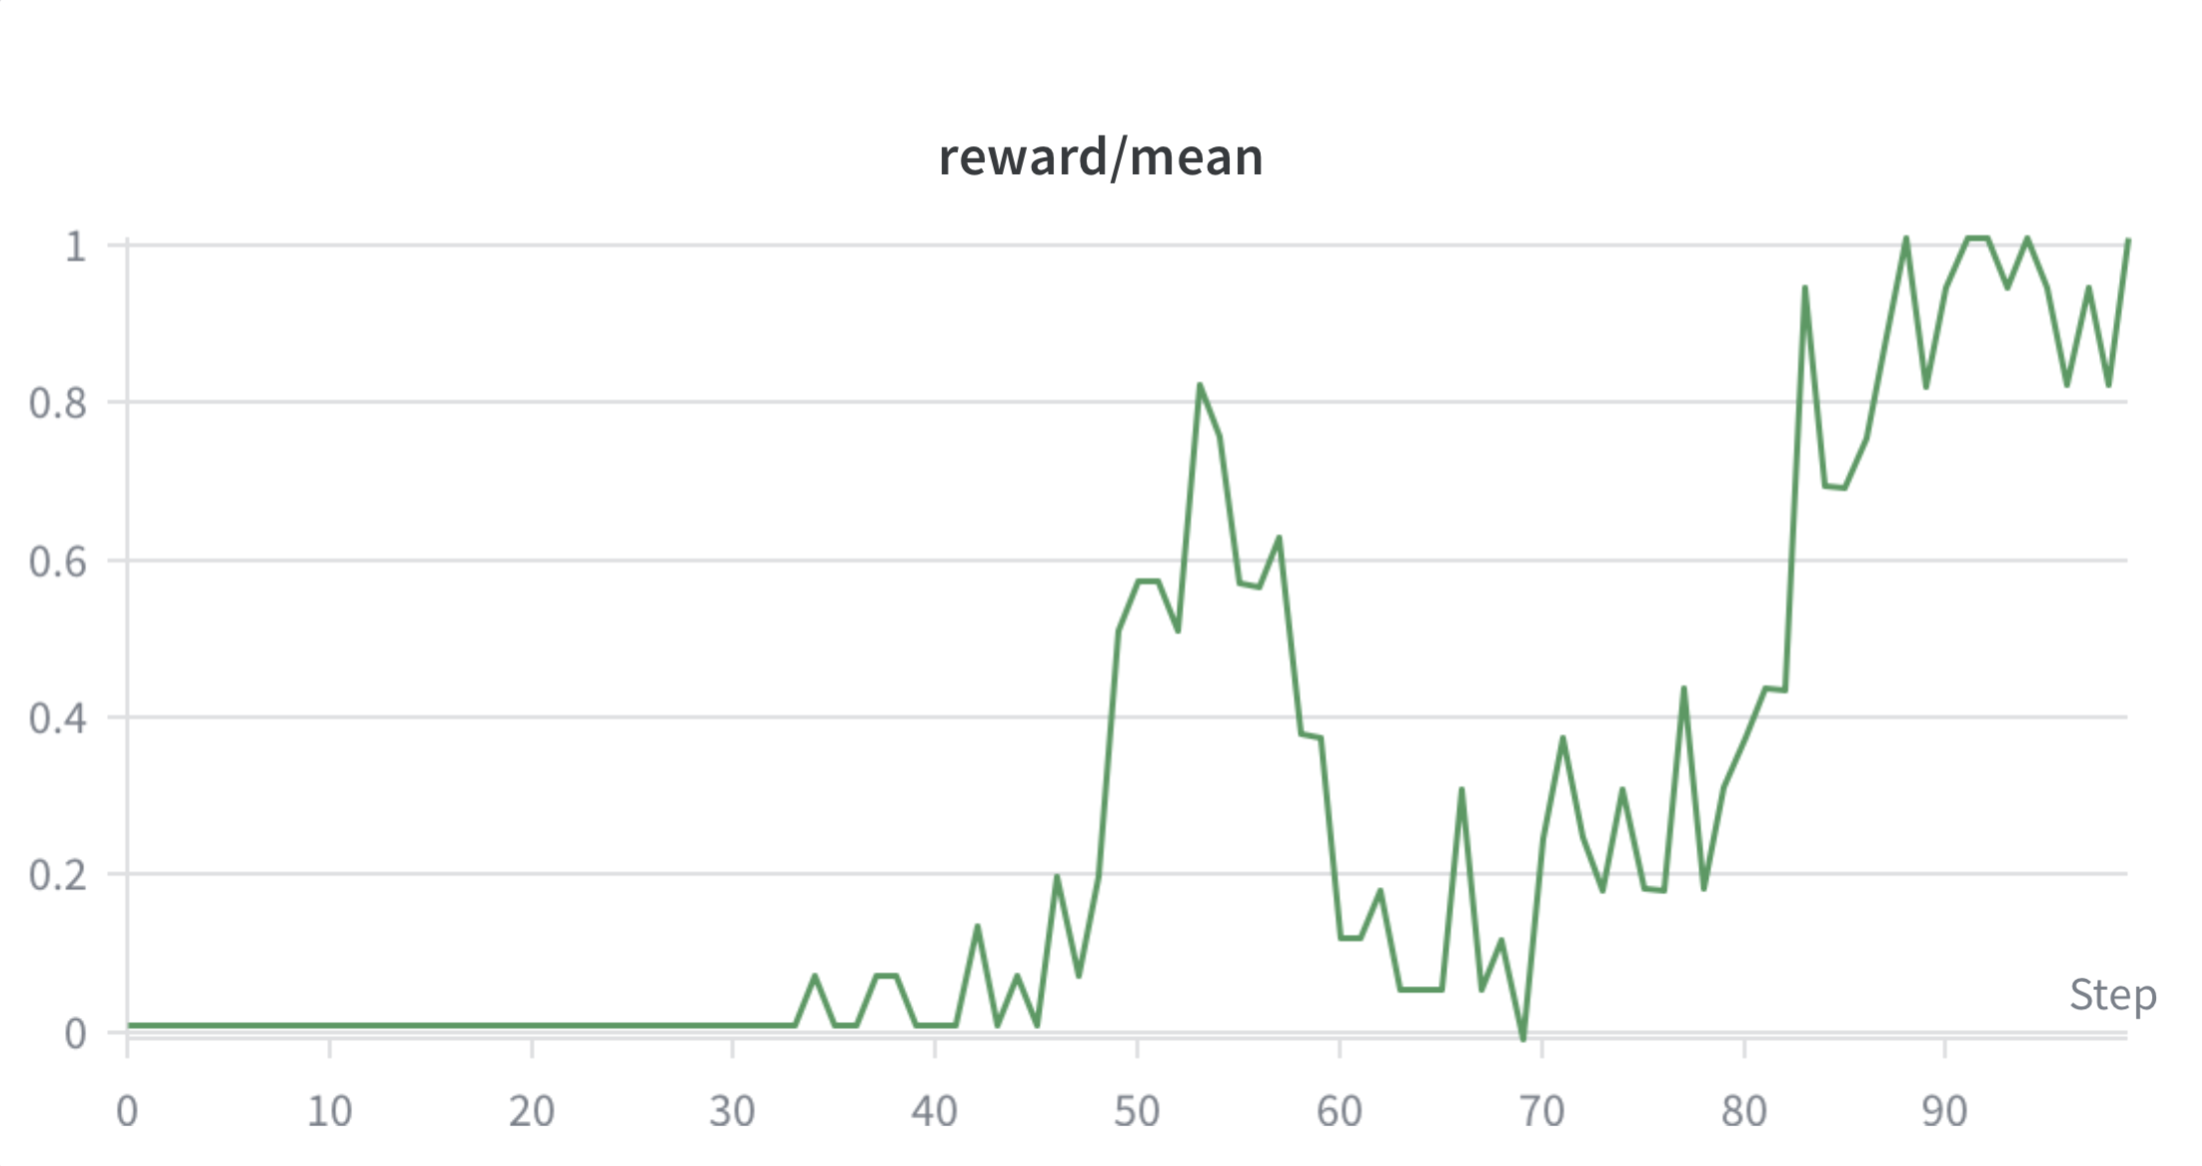
\includegraphics[width=\linewidth]{rewardmean_groundtruth.png}
\end{minipage}
\hfill
\begin{minipage}{0.48\textwidth}
    \centering
    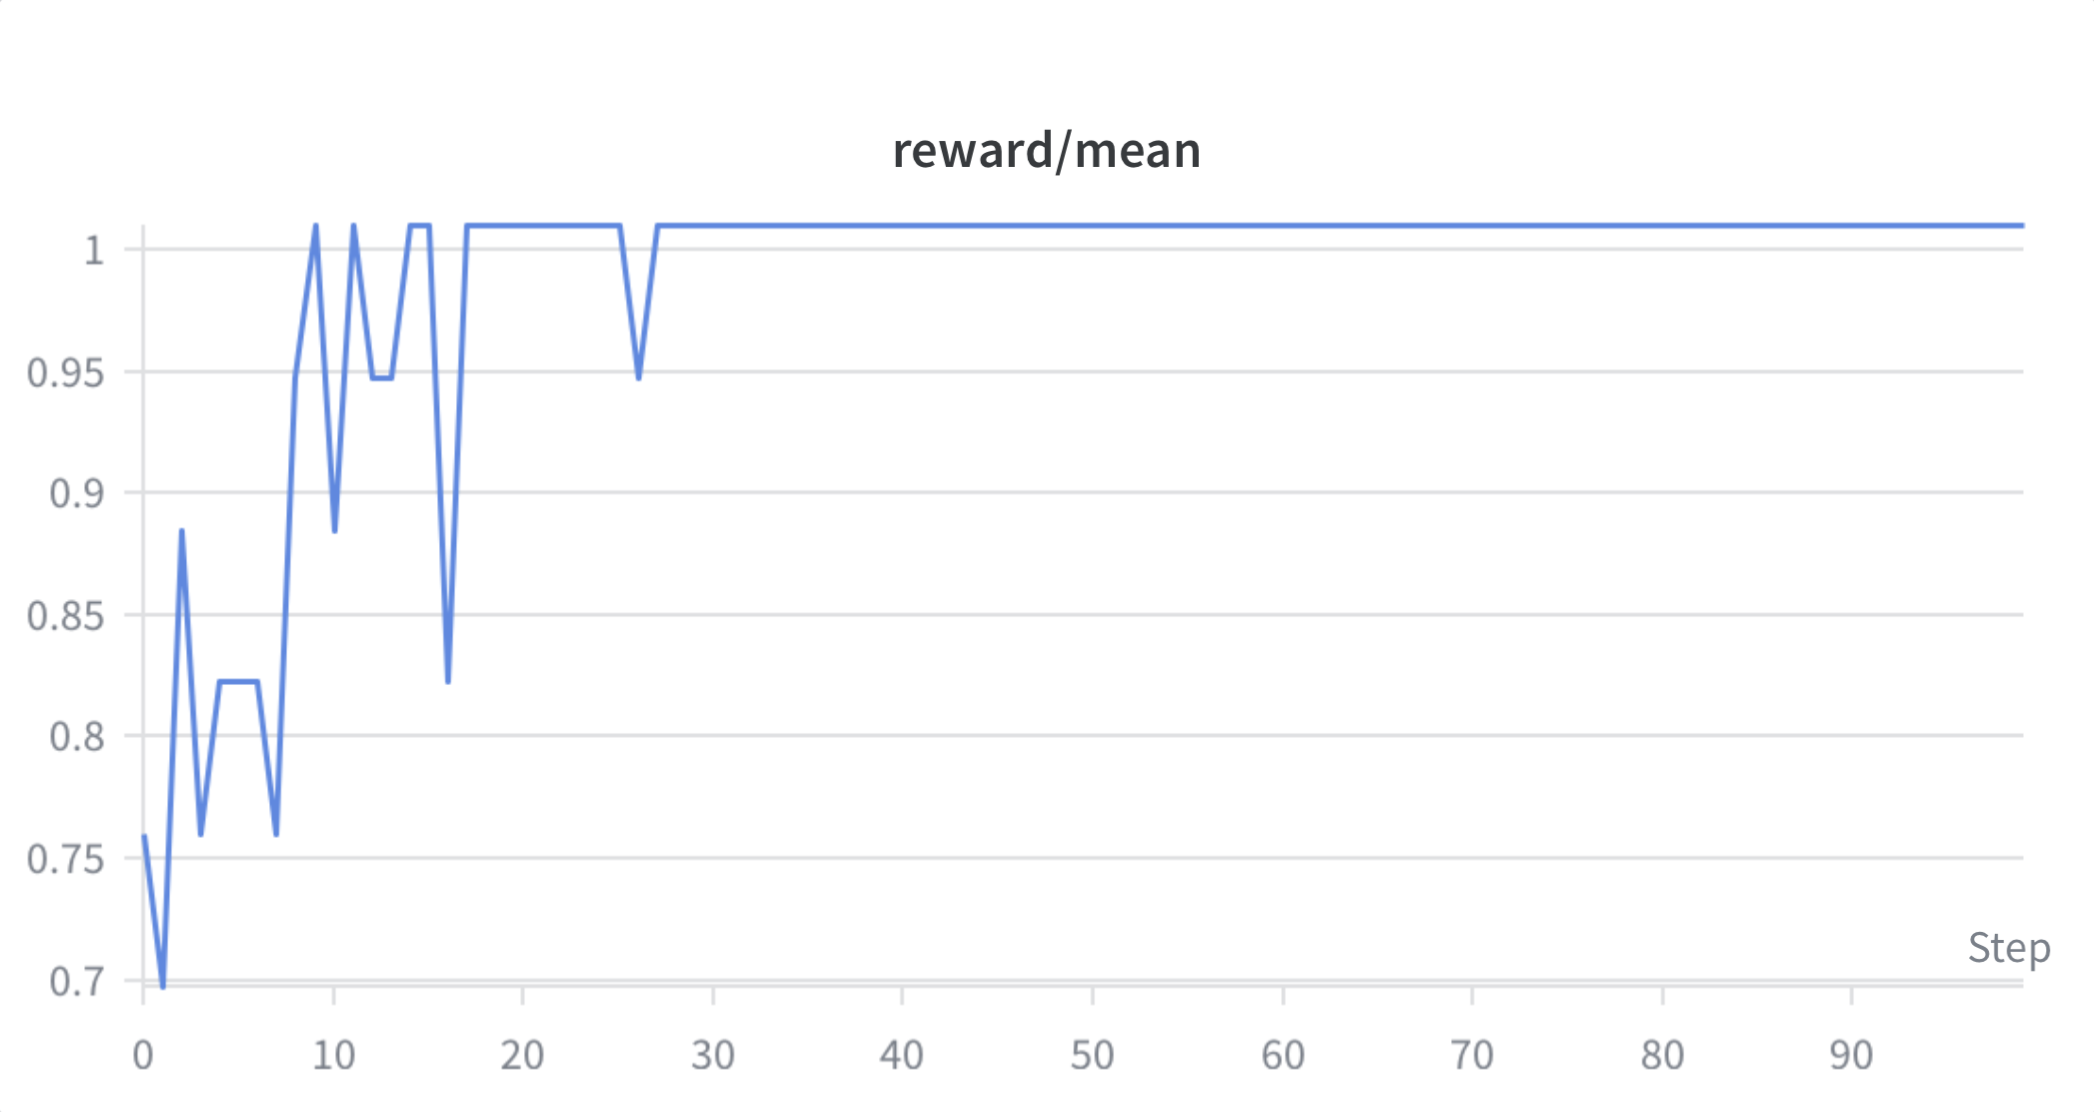
\includegraphics[width=\linewidth]{rewardmean_ttrl.png}
\end{minipage}
\caption{Training reward/mean over 100 steps for both direct GRPO baselines on the target problem. \textbf{Left:} Ground-truth baseline (ref=866). No correct samples appear until step 34, after which GRPO amplifies the rare correct answer to near-unanimous agreement. \textbf{Right:} TTRL consensus baseline (dynamic majority vote). The model's incorrect majority answer (326400) is reinforced from step 0, reaching unanimous agreement by step $\sim$15 and flatlining for the remaining steps.}
\label{fig:baselines}
\end{figure}

These baselines confirm the motivation for our subproblem approach: GRPO \textit{can} learn from extremely sparse correct samples when given ground truth, but without it, consensus-based training on a problem the model cannot solve simply reinforces the wrong answer. Our curriculum of easier subproblems is designed to create the conditions where the model's majority vote is reliable enough to serve as a pseudo-label.

\subsection{Results}

\begin{table}[ht]
\centering
\begin{tabular}{|c|c|c|c|c|c|}
\hline
Step 0 & Step 25 & Step 50 & Step 75 & Step 100 & GPT 5.4 Medium Thinking \\
\hline
0.67\%  & 0.40\% & 9.60\% & \textbf{11.80\%} & 4.20\% & 11.20\%\\
\hline
\end{tabular}
\caption{500-sample solve rate on the target arithmetic geometry problem. The step 0 (unadapted model) solve rate was estimated from 600 samples, while all other solve rates were estimated from 500 samples.}
\label{tab:example}
\end{table}

We did a GRPO training run of 100 steps\footnote{We chose to measure our results in steps instead of epochs. There are two steps in one epoch, so 100 steps corresponds to 50 epochs.} on the 50 valid subproblems, taking checkpoints every 5 steps. We report representative checkpoints at steps 25, 50, 75, and 100 in Table~\ref{tab:example}. For comparison, we also evaluated GPT 5.4 Medium Thinking mode on the same target problem using the same 500-sample solve-rate metric; it solved the problem correctly 56 out of 500 times, corresponding to a solve rate of $11.20\%$.

The baseline \texttt{gpt-oss-120b} model and the step 25 checkpoint performed similarly, at $0.67\%$ and $0.40\%$, respectively, indicating that training had little effect early on. Performance then improved substantially: the step 50 checkpoint reached $9.60\%$, and step 75 achieved the best solve rate of $11.80\%$. Notably, this best checkpoint slightly outperformed GPT 5.4 Medium Thinking, which achieved $11.20\%$ under the same evaluation protocol.

The training trajectory is notably non-monotonic. Although solve rate rises sharply between steps 25 and 75, performance drops to $4.20\%$ by step 100. This suggests that continued optimization does not uniformly improve target-task performance and that intermediate checkpoints may outperform the final model. In this setting, evaluating checkpoints throughout training is therefore important for accurately measuring the benefits of adaptation.

\subsection{Results After Replacing Multi-part Subproblems}

We identified five subproblems in the 50 subproblem training set with multiple questions in the problem statement. Since these subproblems had had multiple questions we replaced them with subproblems that ask for a single answer. After retraining with this cleaned training set to step 50, we found a significant performance boost and a 500-sample solve rate of 30.6\% at step 50. 


\begin{table}[ht]
\centering
\begin{tabular}{|c|c|c|}
\hline
Step 0 & Step 25 & Step 50 \\
\hline
0.67\%  & 9.00\% & \textbf{30.60\%} \\
\hline
\end{tabular}
\caption{500-sample solve rate on the target arithmetic geometry problem. The step 0 (unadapted model) solve rate was estimated from 600 samples, while all other solve rates were estimated from 500 samples.}
\label{tab:example2}
\end{table}

\subsection{Results for Resampling Subproblems at Step 50}

We extended the experiment by training the checkpoint 50 model for an additional 50 steps using subproblems generated by the checkpoint 50 model. First, we resampled 50 new subproblems using the model at checkpoint 50. We then trained again for another 50 steps starting at checkpoint 50, but with a smaller learning rate of $3*10^{-5}$ instead of $1*10^{-4}$. After training again, we found that accuracy remained relatively consistent with a small performance increase of 32.4\% at step 90.  

\begin{figure}
    \centering
    
\includegraphics[width=0.9\linewidth]{template/accuracy_by_step-2.png}
    \caption{Accuracy across training steps}
    \label{fig:placeholder}
\end{figure}



\section{Analysis}
%\lipsum[1][1-9] 

\subsection{Reward-Mean Graph}

\begin{figure}[H]
    \centering
    
\includegraphics[scale=0.6]{template/reward_fn.png}
    \caption{Reward/mean graph during 50 epoch training run}
    \label{fig:your_label}
\end{figure}
The mean reward starts in the mid-70\% range, rises to 80\% by step 10, and fluctuates between 80--90\% for the remainder of training (Figure 1). Two notable drops occur at steps 20 and 70. We attribute these to a tension between skill acquisition and noisy pseudo-labels: as the model learns new reasoning patterns, it may begin producing correct answers that disagree with hallucinated pseudo-labels, causing the reward to drop even as the model's true capability improves.
  
These two drops correspond to markedly different outcomes on the target Tier~3 problem. At step 20, the 500-sample solve rate briefly reaches 1.60\% but collapses back to 0.40\% by step 25, suggesting the acquired skills are fragile and quickly overwritten by continued training against noisy labels. At step 70, however, the solve rate reaches 11.80\% at step 75 and holds at 11.60\% at step 80. The persistence of these gains suggests that by this point in training, the model has internalized deeper reasoning strategies that are robust to subsequent label noise. Together, these results confirm that the subproblem curriculum transfers meaningful skills to the target problem, while also highlighting hallucinated pseudo-labels as a key limitation: they can partially reverse early gains, though sufficiently deep learning appears to survive.

\subsection{Pseudo-label reliability}

We also analyzed the reliability of the pseudo-labels used to train GRPO on the 50 selected subproblems. Each pseudo-label was produced by self-consistency on \texttt{gpt-oss-120b}: we sampled 10 solutions, took the most frequent final numerical answer, and used that modal answer as the reference label whenever its frequency fell within our acceptance range.

To estimate how often these pseudo-labels were actually correct, we constructed a stronger external reference signal. For each of the 50 selected subproblems, we sampled one response from each of three frontier models: Claude Opus 4.6 Extended Thinking, Gemini 3.1 Pro, and GPT 5.4 Thinking (xhigh). We then took the majority-vote final numerical answer across these three models and treated it as an approximate reference label. We compared this frontier-model consensus answer against the pseudo-label assigned by \texttt{gpt-oss-120b} self-consistency.

Across the 50 selected subproblems, the pseudo-label agreed with the frontier-model majority vote on only $50\%$ of problems. Under this proxy evaluation protocol, the estimated pseudo-label error rate is therefore approximately $50\%$. This suggests that while self-consistency is useful for identifying subproblems near the model's learning frontier, it is much less reliable as a guarantee that the assigned label is correct.

Our follow-up inspection suggests that the issue is not only noisy pseudo-labels, but also the quality of the generated subproblems themselves. Some subproblems appeared to be poorly formed or to contain inconsistent premises, which can naturally produce disagreement across strong models even when each model is reasoning coherently. In other cases, an apparent majority answer was unstable: after exposing models to alternative reasoning, frontier models sometimes revised their answers, suggesting that simple answer agreement may overstate confidence in the reference label. These observations indicate that errors can arise both from incorrect pseudo-labeling and from the generation of subproblems that are not well-posed.

Taken together, these findings point to subproblem quality as a major bottleneck in our pipeline. Future improvements should therefore focus on generating better-posed and more internally consistent subproblems before training on them.

At the same time, it is notable that GRPO still improved target-problem performance despite this high estimated pseudo-label error rate. This suggests that the training procedure is somewhat robust to noisy supervision: even imperfect subproblems may still teach useful intermediate skills. Nevertheless, improving pseudo-label reliability and subproblem quality remains an important direction for future work.


\subsection{Recovery from incorrect pseudo-labels}

We also observed an instructive failure case in which the model appeared to recover from an incorrect pseudo-label during training. At step 95, we examined one of the sampled enumerative geometry subproblems listed in the Appendix \ref{sec:Appendix}.

The pseudo-label assigned earlier in our pipeline was 7200. However, external frontier-model checking suggested that this reference answer was likely incorrect: both GPT 5.4 Thinking Medium and Claude Opus 4.6 Extended Thinking gave 100 as the answer.

What makes this example notable is that when we sampled 16 rollouts from the trained model on this subproblem at step 95, the model produced the answer 100 in 10 out of 16 samples, exceeding the frequency of the pseudo-label 7200. In other words, the model's own output distribution had shifted toward the answer that the stronger external models supported, despite the fact that the training reference label was wrong.

This suggests that GRPO training in our setting is not merely memorizing or rigidly amplifying noisy pseudo-labels. Instead, the model may sometimes learn intermediate structure from the subproblem that allows the correct answer to dominate the sampled rollouts even when the original supervision is flawed. Although this is only a single case study, it is encouraging evidence that the training process may have some robustness to pseudo-label noise.


\section{Conclusion}
We present a curriculum-based approach to test-time training for solving problems in binary reward settings. By prompting the model to generate easier subproblems, filtering them via self-consistency, and training with GRPO, we improved the solve rate on a Tier~3 Frontier-Math arithmetic geometry problem from 0.67\% to 30.6\%---a roughly $46\times$ improvement---without any ground-truth labels for the intermediate tasks. This result substantially outperforms GPT-5.4 Medium Thinking (11.20\%) under the same evaluation protocol. We further showed that resampling subproblems from the improved checkpoint and continuing training yields additional gains, reaching 32.4\% at step 90, demonstrating that iterative curriculum refinement can extract further performance.
 
Our analysis revealed both the promise and the limitations of this approach. On the positive side, the subproblem curriculum restored meaningful gradient signal where direct RL on the target problem would have produced none, and the model demonstrated some capacity to recover from incorrect pseudo-labels during training. We also found that subproblem quality matters significantly: replacing five multi-part subproblems with single-answer variants nearly tripled the solve rate from 11.80\% to 30.6\%, highlighting the importance of well-posed training tasks. On the other hand, pseudo-label reliability remains a significant bottleneck: approximately 50\% of our assigned labels disagreed with frontier-model consensus, and the non-monotonic training trajectory suggests that noisy supervision can partially erode gains at later steps.
 
These findings point to several directions for future work. First, improving subproblem generation---for instance, by incorporating formal verification or iterative refinement to ensure problems are well-posed and single-valued---could substantially reduce label noise, as our multi-part subproblem ablation suggests. Second, iterative resampling of subproblems from improved checkpoints is a promising strategy for continued gains, though our initial results suggest diminishing returns with a single round of resampling. Third, adaptive checkpoint selection during training could help capture peak performance before overfitting to noisy labels. Finally, scaling this approach across multiple problems and domains would test whether curriculum-based test-time training generalizes beyond the single-problem setting studied here.

\section*{Team contributions (Required for multi-person team)}
% \lipsum[1][1-3] 

Darrow -  Model Training, subproblem generation pipeline, model evaluation scripts, xhigh thinking
\\Leo - Model Training, Big Thinking, Analyzing pseudo-labels, evaluating model performance, etc. 
\\ Andrew - Explored retrosynthesis (prior to pivot), gathered data, model training

\bibliographystyle{unsrt}
\bibliography{references}

% \appendix

\section{Appendix}
\label{sec:Appendix}

\begin{center}
\setlength{\fboxsep}{14pt}
\fcolorbox{gray!35}{gray!10}{%
\parbox{0.94\textwidth}{%

\vspace{1em}

\textbf{\large Subproblem:}
Consider the projective space \(\mathbb{P}^5\) over an algebraically closed field of characteristic \(0\), with homogeneous coordinates \([z_0:\dots:z_5]\). Let \(Q_1,Q_2,Q_3\) be three generic homogeneous quadratic polynomials and \(C_1,C_2\) be two generic homogeneous cubic polynomials in these variables. Define the zero-dimensional scheme
\[
X = \{[z]\in \mathbb{P}^5 \mid Q_1([z]) = Q_2([z]) = Q_3([z]) = C_1([z]) = C_2([z]) = 0\}.
\]
Let \(\mathcal{Q}\) be the parameter space of ordered \(5\)-tuples \((Q_1,Q_2,Q_3,C_1,C_2)\) of such polynomials (each up to scaling), which is a dense open subset of a product of projective spaces. Define the incidence variety
\[
Z = \{(x,\mathbf{Q}) \in \mathbb{P}^5 \times \mathcal{Q} \mid x \text{ satisfies all five equations of } \mathbf{Q}\}
\]
and let \(\pi : Z \to \mathcal{Q}\) be the projection onto the second factor. Over a dense open subset \(V\subset \mathcal{Q}\), the map \(\pi\) is finite étale. Define
\[
L = \lim_{p\to\infty} \frac{1}{\#V(\mathbb{F}_p)} \sum_{\mathbf{Q}\in V(\mathbb{F}_p)} \#\pi^{-1}(\mathbf{Q}).
\]
Compute \(\lfloor 100L \rfloor\).
}%
}
\end{center}

\end{document}
